\begin{figure}[!ht] \label{gig:bib}
\centering

\tikzstyle{process} = [rectangle, minimum width=1.5cm, minimum height=6.5cm, text centered, draw=black, fill=white, text width=1.75cm, font=\small]
\tikzstyle{mid_process} = [rectangle, minimum width=1cm, minimum height=1cm, text centered, draw=black, fill=white, text width=1.75cm, font=\small]
\tikzstyle{arrow} = [thick,->,>=stealth]

\scalebox{0.7}{%
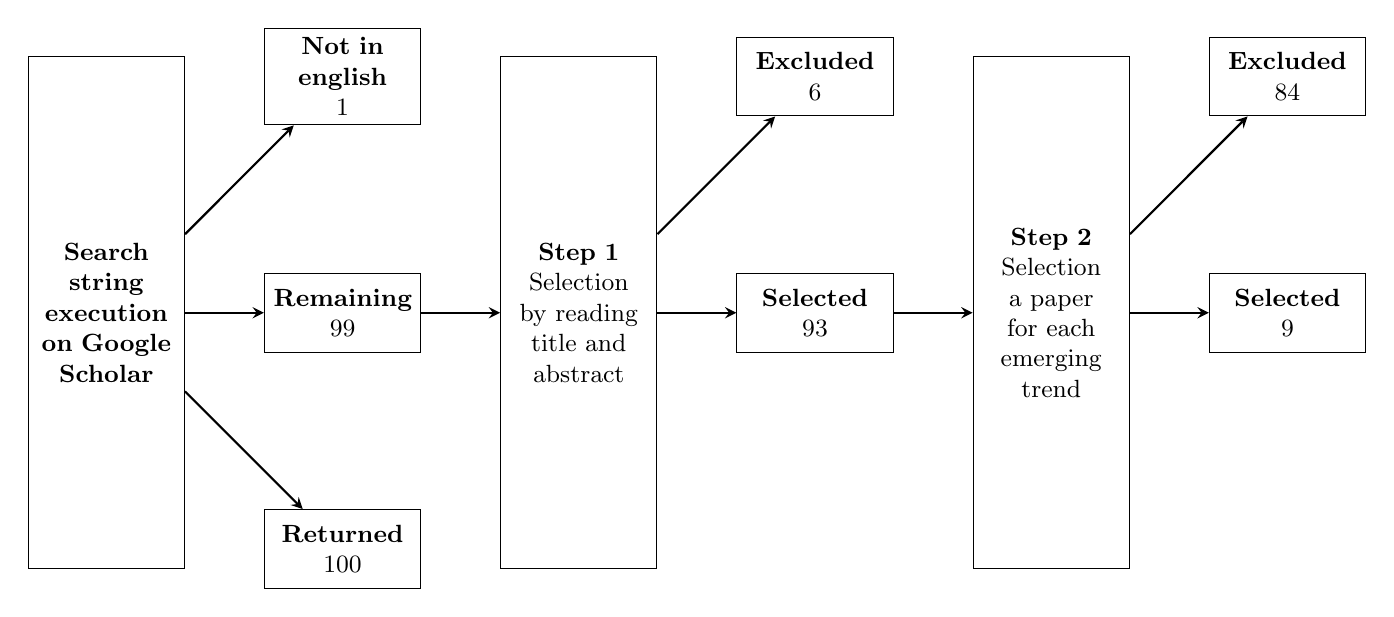
\begin{tikzpicture}[node distance=3cm, auto]

    % Nodes
    \node (start) [process] {\textbf{Search string execution on Google Scholar}};
    \node (remaining) [mid_process, right of=start] {\textbf{Remaining} \\ 99};
    \node (repeat) [mid_process, above of=remaining] {\textbf{Not in english} \\ 1};
    \node (returned) [mid_process, below of=remaining] {\textbf{Returned} \\ 100};
    
    \node (step1) [process, right of=remaining] {\textbf{Step 1} \\ Selection by reading \\ title and abstract};
    \node (included1) [mid_process, right of=step1] {\textbf{Selected} \\ 93};
    \node (excluded1) [mid_process, above of=included1] {\textbf{Excluded} \\ 6};


    \node (step2) [process, right of=included1] {\textbf{Step 2} \\ Selection a paper for each \\ emerging trend};
    \node (included2) [mid_process, right of=step2] {\textbf{Selected} \\ 9};
    \node (excluded2) [mid_process, above of=included2] {\textbf{Excluded} \\ 84};

    % Arrows
    \draw [arrow] (start) -- (remaining);
    \draw [arrow] (start) -- (repeat);
    \draw [arrow] (start) -- (returned);
    
    \draw [arrow] (remaining) -- (step1);
    \draw [arrow] (step1) -- (excluded1);
    \draw [arrow] (step1) -- (included1);

    
    \draw [arrow] (included1) -- (step2);
    \draw [arrow] (step2) -- (excluded2);
    \draw [arrow] (step2) -- (included2);
    

\end{tikzpicture}
}

\caption{Selection Process of the Articles.}
\label{fig:bib}
\end{figure}